\documentclass[11pt]{article}
\usepackage{amsmath,amssymb,amsthm}
\usepackage[utf8]{inputenc}
\usepackage{graphicx}
\usepackage{xcolor}

\DeclareMathOperator*{\E}{\mathbb{E}}
\let\Pr\relax
\DeclareMathOperator*{\Pr}{\mathbb{P}}

\newcommand{\eps}{\varepsilon}
\newcommand{\inprod}[1]{\left\langle #1 \right\rangle}
\newcommand{\R}{\mathbb{R}}

\theoremstyle{definition} \newtheorem{Theorem}{theorem}

\newcommand{\handout}[5]{
  \noindent
  \begin{center}
  \framebox{
    \vbox{
      \hbox to 6.38in { \textcolor{black}{\bf CS 134: Networks } \hfill #4  }
      \vspace{1mm}
      \hbox to 6.42in { #3 {\hfill #2 } }
      \vspace{0.0mm}
      \hbox to 6.38in { { \hfill} }
    }
  }
  \end{center}
  \vspace*{0mm}
}

\newcommand{\pset}[3]{\handout{{#1}}{\textcolor{red}{Due: #2}}{\textcolor{black}{#3}}{\textcolor{gray}{\textbf{Problem set #1}}}}

\newtheorem{theorem}{Theorem}
\newtheorem{corollary}[theorem]{Corollary}
\newtheorem{lemma}[theorem]{Lemma}
\newtheorem{observation}[theorem]{Observation}
\newtheorem{proposition}[theorem]{Proposition}
\newtheorem{definition}[theorem]{Definition}
\newtheorem{claim}[theorem]{Claim}
\newtheorem{fact}[theorem]{Fact}
\newtheorem{assumption}[theorem]{Assumption}
\newtheorem{remark}[theorem]{Remark}

\newtheorem*{theorem*}{Theorem}
\newtheorem*{notation*}{Notation}
\newtheorem*{assumption*}{Assumption}
\newtheorem*{fact*}{Fact}
\newtheorem*{claim*}{Claim}
\newtheorem*{definition*}{Definition}
\newtheorem*{exercise*}{Exercise}
\newtheorem*{lemma*}{Lemma}
\newtheorem*{remark*}{Remark}

% 1-inch margins, from fullpage.sty by H.Partl, Version 2, Dec. 15, 1988.
\topmargin 0pt
\advance \topmargin by -\headheight
\advance \topmargin by -\headsep
\textheight 8.9in
\oddsidemargin 0pt
\evensidemargin \oddsidemargin
\marginparwidth 0.5in
\textwidth 6.5in

\parindent 0in
\parskip 1.5ex


\usepackage[margin=.9in]{geometry}
\usepackage{amsmath}
\usepackage{tikz}
\usepackage{float}
\usepackage{filecontents}
\usepackage{pgfplots, pgfplotstable}
\usepackage{listings}

%\usepgfplotslibrary{statistics}
\usepackage[T1]{fontenc}
%\usepackage{enumitem}
\usepackage{hyperref}
\usetikzlibrary{calc,intersections,through,backgrounds,shadings}
\usetikzlibrary{shapes.geometric}
\usetikzlibrary{through}

\usepackage[nofiglist,nomarkers]{endfloat}
\renewcommand{\efloatseparator}{\mbox{}}

\usepackage{exercise}
\renewcommand{\ExerciseHeader}{{ \textbf{
\ExerciseName \ \ExerciseHeaderNB \ExerciseHeaderTitle
\ExerciseHeaderOrigin.}}}

\usepackage{pgfplots}
\pgfplotsset{
%  compatgraph=newest,
  xlabel near ticks,
  ylabel near ticks
}



\begin{document}

\pset{4}{\textbf{Wednesday 3/1/2017}}{{Prof.\ Yaron Singer}}

\paragraph{1. Centrality (Jackson 2.2.4).}
 \par
 The \emph{degree centrality} of a node is its degree divided by $n-1$ (where $n$ is the number of nodes in the network). For example, the degree centrality of node $d$ in network $A$ (see appendix) is $\frac{3}{5}$.

 \begin{itemize}
\item[\textbf{a.}] Compute the degree centrality of each of the nodes in network $B$. 
 \end{itemize} \emph{Closeness Centrality}.
 The most basic closeness centrality measure is the inverse of the average distance between $i$ and all other nodes $j$ in the network\footnote{There are various conventions for handling networks that are not connected, as well as other possible measures of distance, which lead to a family of closeness measures, but for now we won't get into this.}. To illustrate, let us compute the closeness centrality of node $b$ in the following network $$(\{a,b,c\},\{ab,ac\}).$$
 
 \begin{itemize}
 \item The distance between node $b$ and node $a$ is $1$.
 \item The distance between node $b$ and node $c$ is $2$.
\end{itemize}

The average of these distances is $\frac{3}{2}$, so the closeness centrality of node $b$ in this network is $\frac{2}{3}$.
 
\begin{enumerate} 
\item[\textbf{b.}]Compute the closeness centrality of node $d$ in network  $$(\{a,b,c,d\},\{ab,ac,ad,bc,cd\}).$$ \end{enumerate}
 

\paragraph{2. Betweenness Centrality.}
 Let $P_i(k,j)$ denote the number of geodesics (or shortest paths) between nodes $k$ and $j$ that node $i$ lies on, and let $P(k,j)$ be the total number of geodesics between nodes $k$ and $j$. We can estimate how important node $i$ is in terms of connecting nodes $k$ and $j$ by looking at the fraction $\frac{P_i(k,j)}{P(k,j)}$ of shortest paths between nodes $k$ and $j$ that involve node $i$. Averaging this ratio across all pairs of nodes (aside from node $i$) gives us the \emph{betweeness centrality} of node $i$. To illustrate, let us compute the betweenness centrality of node $c$ in the following ``circle network'' $$(\{a,b,c,d\}, \{ab,bc, cd,da\}).$$ 
  
\begin{itemize}
 \item None of the shortest paths between node $a$ and node $b$ involve node $c$, so $\frac{P_c(a,b)}{P(a,b)}=0$.
  \item None of the shortest paths between node $a$ and node $d$ involve node $c$, so $\frac{P_c(a,d)}{P(a,d)}=0$.  
 \item One of the two shortest paths between nodes $b$ and node $d$ involve node $c$, so $\frac{P_c(b,d)}{P(b,d)}=\frac{1}{2}$.
\end{itemize}


Averaging out these three ratios, we find that the betweenness centrality of node $c$ in this network is $\frac{1}{6}$.
 
Compute the betweenness centrality of each of the nodes in the network $(\{a,b,c,d,e,f\}, \{ab,bc,cd,ce,df,ef\})$. 


\paragraph{3. Programming: Verifying the Friendship Paradox.}  Using the eight sample directed social networks below, courtesy of \href{https://snap.stanford.edu/data}{SNAP} (https://snap.stanford.edu/data), for each social network, compute the value of
$$\frac{\frac{1}{|G|}\sum\limits_{n \in G}(deg(n))}{\frac{1}{|G|}\sum\limits_{n\in G}(\frac{1}{|N(n)|}\sum\limits_{m \in N(n)} deg(m))}$$
with the average being taken across all nodes $n$ in the network $G$, and where $N(n)$ is the neighborhood of node $n$.

(That is, calculate the value of ($\text{average node degree}/\text{average average degree of node's neighbors}$) in the graph.)

If the networks are too large, consider a reasonable (what constitutes "reasonable" is up to your judgment, as long as you provide a textual defense in your submission) subsample of the nodes.

Keep in mind that the graph is directed, only consider outgoing edges when computing degree, and only consider neighbors to whom node $n$ has an outgoing edge to that neighbor. If a node has out-degree of $0$, then assume the average degree of its neighbors is $0$. \\

Compute the value above for each of the following social networks: \begin{itemize}
\item \href{https://snap.stanford.edu/data/com-Orkut.html}{https://snap.stanford.edu/data/com-Orkut.html}
\item \href{https://snap.stanford.edu/data/com-LiveJournal.html}{https://snap.stanford.edu/data/com-LiveJournal.html}
\item \href{https://snap.stanford.edu/data/soc-Slashdot0811.html}{https://snap.stanford.edu/data/soc-Slashdot0811.html}
\item \href{https://snap.stanford.edu/data/com-DBLP.html}{https://snap.stanford.edu/data/com-DBLP.html}
\item \href{https://snap.stanford.edu/data/email-Enron.html}{https://snap.stanford.edu/data/email-Enron.html}
\item \href{https://snap.stanford.edu/data/com-Youtube.html}{https://snap.stanford.edu/data/com-Youtube.html}
\item \href{https://snap.stanford.edu/data/soc-Epinions1.html}{https://snap.stanford.edu/data/soc-Epinions1.html}
\item \href{https://snap.stanford.edu/data/wiki-Talk.html}{https://snap.stanford.edu/data/wiki-Talk.html}
\end{itemize}

You should use the first dataset in the `Files' table on each page. Note that some of these graphs are directed, and some are undirected, as indicated by 'ungraph', which you should account for when building the graphs.

As a \textbf{bonus question (just for fun, no extra credit)}, for each network, plot the average of $\frac{deg(n)}{\frac{1}{|N(n)|}\sum\limits_{m \in N(n)} deg(m)}$ against sample size (number of nodes $n$ in the subsample). That is, for samples of varying sizes, compute this average for each sample on the $y$ axis, and plot the sample size on the $x$ axis.

You should also turn in to Canvas a script named `\textit{Lastname\_Firstname\_ps4.py}', with your name substituted in place of `\textit{Lastname\_Firstname}', in addition to the rest of your problem set, and the appropriate extension for the language you're using. If you are using python, see \href{https://piazza.com/class/iy4iludwvo851z?cid=269}{this Piazza link (post 269)} for expectations on how to submit your code (specifically: we'll no longer accept python notebooks in submission, though they're fine to use while solving the problem).



%%%%%%%%%%% Network A
\begin{figure}[t] 
\centering
\caption{Network $A$}
\label{example}
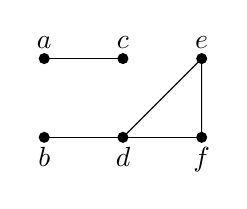
\begin{tikzpicture} [scale=1]

\coordinate [label=above:{$a$}] (a) at (0,1);
\coordinate [label=below:{$b$}] (b) at (0,0);
\coordinate [label=above:{$c$}] (c) at (1,1);
\coordinate [label=below:{$d$}] (d) at (1,0);
\coordinate [label=above:{$e$}] (e) at (2,1);
\coordinate [label=below:{$f$}] (f) at (2,0);

\fill (a) circle (2pt);
\fill (b) circle (2pt);
\fill (c) circle (2pt);
\fill (d) circle (2pt);
\fill (e) circle (2pt);
\fill (f) circle (2pt);

\draw (a)--(c);
\draw (d)--(e)--(f);
\draw (b)--(d)--(f);

\end{tikzpicture}
\end{figure}

%%%%%%%%% Network B
\begin{figure} 
\centering
\caption{Network $B$}
\label{exercise}
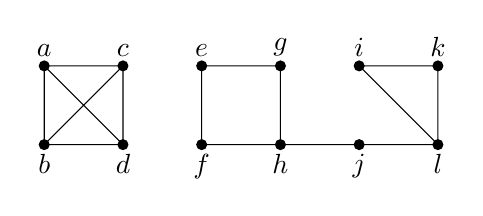
\begin{tikzpicture} [scale=1]

\coordinate [label=above:{$a$}] (a) at (0,1);
\coordinate [label=below:{$b$}] (b) at (0,0);
\coordinate [label=above:{$c$}] (c) at (1,1);
\coordinate [label=below:{$d$}] (d) at (1,0);
\coordinate [label=above:{$e$}] (e) at (2,1);
\coordinate [label=below:{$f$}] (f) at (2,0);
\coordinate [label=above:{$g$}] (g) at (3,1);
\coordinate [label=below:{$h$}] (h) at (3,0);
\coordinate [label=above:{$i$}] (i) at (4,1);
\coordinate [label=below:{$j$}] (j) at (4,0);
\coordinate [label=above:{$k$}] (k) at (5,1);
\coordinate [label=below:{$l$}] (l) at (5,0);

\fill (a) circle (2pt);
\fill (b) circle (2pt);
\fill (c) circle (2pt);
\fill (d) circle (2pt);
\fill (e) circle (2pt);
\fill (f) circle (2pt);
\fill (g) circle (2pt);
\fill (h) circle (2pt);
\fill (i) circle (2pt);
\fill (j) circle (2pt);
\fill (k) circle (2pt);
\fill (l) circle (2pt);

\draw (a)--(d)--(c)--(b)--(a)--(c)--(d)--(b);
\draw (h)--(f)--(e)--(g)--(h)-- (j)--(l)--(k)--(i)--(l);

\end{tikzpicture}
\end{figure}




\end{document}

pdflatex pset 2. Basic Graph Theory.tex

